\documentclass[titlepage]{article}
\usepackage[utf8]{inputenc}
\usepackage[margin=1in]{geometry}
\usepackage{graphicx}
\usepackage{enumitem}
\usepackage{placeins}
\usepackage{dirtree}
\usepackage{enumitem,amssymb}
\newlist{todolist}{itemize}{2}
\setlist[todolist]{label=$\square$}
\usepackage{multicol}
\usepackage{cprotect}

\newlist{steps}{enumerate}{1}
\setlist[steps, 1]{label = Step \arabic*:}

\title{\Huge Groundhog Radar System Operation and Maintenance Manual}
\author{\LARGE Michael Christoffersen}
\date{\LARGE April 2023\\v1.0}

\begin{document}

\maketitle

\tableofcontents

\pagebreak

\section{Setup \& Operation}
\subsection{Setup}
\begin{enumerate}[1.]
    \item Lay out four antenna elements. Usually this is done in an endfire orientation that looks like this ( | | ) as opposed to a broadside orientation ( $\mid \hspace{1em} \mid$ ). A broadside orientation could cause significant coupling between the two antennas, leading to excess ringing.
    \item Set up the transmitter (pulser):
    \begin{enumerate}[(a)]
        \item Connect the two tansmit antenna elements to the ``-ve'' and ``+ve'' ports.
        \item Connect a 12v battery to the ``DC power in'' ports.
        \item \textbf{Note}: Sometimes the pulser fails to begin pulsing when the power is connected so be sure to check that yellow ``Active'' light is on when the power is connected. If it is not you should disconnect the reconnect power.
        \item \textbf{Note}: It is best to connect the antenna elements before powering the transmitter to avoid a chance of a significant shock.
    \end{enumerate}
    
    \item Set up the receiver hardware \begin{enumerate}[(a)]
        \item Connect the two antenna elements to a BNC-banana jack adapter.
        \item Connect the BNC-banana jack adapter to the balanced port of a balun.
        \item Connect the unbalanced port of the balun to an anti-alias filter (something in the neighborhood of 10 MHz if you are digitizing at 20 MHz).
        \item Optional: add a pre-amplifier (and probably an RF limiter too) after the filter. \textbf{Note}: This is likely not necessary and potentially harmful to data quality for glaciers less than 600m thick.
        \item Use a BNC-SMA adapter if necessary to connect to the RF 1 port on the USRP N210.
        \item Ensure the USRP N210 (the radio) is powered. It should be supplied with 6v, either with a voltage regulator of some sort or a 6v battery.
        \item Connect the ethernet port of the USRP N210 to the ethernet port of the field laptop. 
        \item Connect the Garmin USB GPS to a USB port of the field laptop. 
        \item \textbf{Note}: Connecting USB devices other than the Garmin GPS to the field laptop can potentially prevent communication with the GPS, so that should be avoided.
    \end{enumerate}

    \item Verify operation of the transmitter and receiver \begin{enumerate}[(a)]
        \item Open a terminal window on the field laptop and navigate to the directory \\\verb+/home/radar/groundhog/control+.
        \item Run the GPS test script, \verb+./gps-test.sh+. after a 5 second delay it will print out 4 or 5 GPGGA sentences if the Garmin GPS is communicating properly with the field laptop. If there are no GPGGA sentences printed see the GPS troubleshooting section of this document (\ref{trouble_gps}) 
        \item Run the receiver test script, \verb+./plot_rx.py+. It will record and plot one tenth of a second of samples. If no plot is generated see the USRP N210 troubleshooting section of this document (\ref{trouble_usrp}). The plot should appear somewhat similar to Figure \ref{fig:plot_rx} although your ambient noise level may significantly vary. If the plot only appears to have noise see the transmitter and antenna troubleshooting sections of this document (\ref{trouble_xmit}, \ref{trouble_ant}).
        \item Use the \verb+plot_rx.py+ plot to decide on a trigger threshold. Keep in mind that the trigger works on absolute amplitude, so a positive or negative polarity signal with a larger amplitude than the trigger threshold will cause a trigger. An appropriate trigger threshold for the signal in Figure \ref{fig:plot_rx} would be 2000 counts.
    \end{enumerate}

    \item Once you have verified operation of the transmitter and receiver you almost ready to acquire data (!). Change the trigger threshold in \verb+run_radar.sh+ to the value you chose from inspecting the plot generated by \verb+plot_rx.py+. You can use gedit, \verb+gedit run_radar.sh+, or your favorite terminal text editor. Make sure to save and close the file when you are finished. Now you are ready to acquire data.
\end{enumerate}

\begin{figure}[h]
\centering
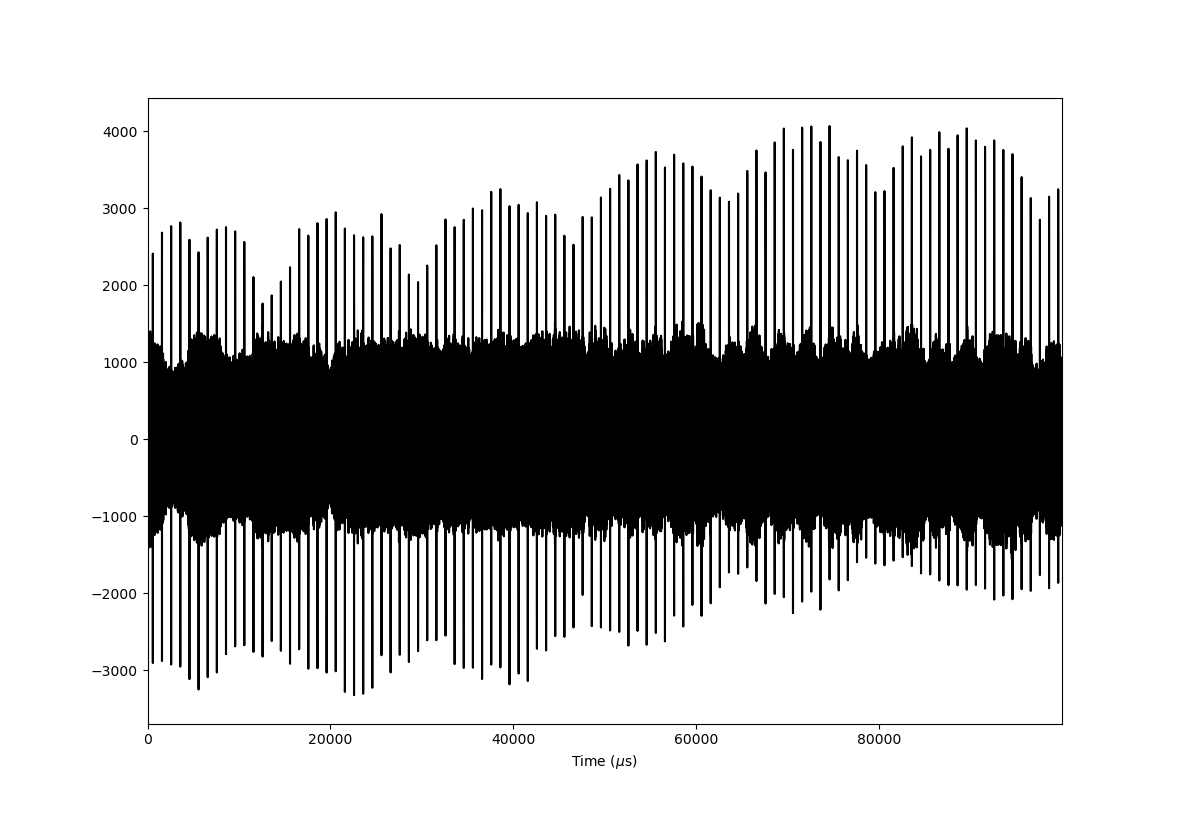
\includegraphics[width=\textwidth]{figs/plot_rx.png}
\cprotect\caption{An example of the graph produced by \verb:plotRX.py: when the transmitter and receiver are working properly. The positive and negative polarity amplitude spikes (to roughly +/- 3500 counts) are the transmitter pulses. The darker region of the plot is ambient noise and reflected pulses.}
\label{fig:plot_rx}
\end{figure}

\subsection{Operation}
The \verb+run_radar.sh+ script operates the radar. It generates an unused filename, \verb|groundhogXXXX| (between \verb+groundhog0000+ and \verb+groundhog9999+) and then starts \verb+gpspipe+ logging NMEA sentences to the file \verb|groundhogXXXX.txt|. Then it starts the digitizer software which begins logging to \verb|groundhogXXXX.dat|.

You'll run \verb|./run_radar| to begin data acquisition and then use \verb|Ctrl+c| to end it. The GPS and radar data files will be saved in the directory \verb|/home/radar/groundhog/data|.

\subsection{Processing}
The processing pipeline is small, all files are in \verb|/home/radar/groundhog/process|. The \verb|ghog2h5.py| script converts files from the groundhog digitizer format to HDF5. It is hardcoded to go look for files ending in \verb|.dat| in the directory \verb|/home/radar/groundhog/data| and can be run without any arguments. The script \verb|makeQlook.py| generates quicklook images of the data inside each HDF5 file. It is hardcoded to go look for files ending in \verb|.h5| in the directory \verb|/home/radar/groundhog/data| and can be run without any arguments.

\section{Troubleshooting}
\subsection{GPS} \label{trouble_gps}
The GPS logging uses \verb|gpsd| to do the heavy lifting of communicating with the USB GPS. In \verb|run_radar.sh| the program \verb|gpspipe| is used to direct the real time output of the USB GPS to a file. If the GPS is not communicating with the computer for some reason the solution is likely a power cycle. The program \verb|gpsmon| can be run in the terminal to see the real-time output of the USB GPS. If there is no GPS information being received \verb|gpsmon| will show some JSON strings and nothing else. If there is GPS information being received \verb|gpsmon| will show a rectangular window with a GPS fix.

\subsection{USRP N210} \label{trouble_usrp}


\subsection{Kentech Pulser} \label{trouble_xmit}
There is not a lot that can go wrong with the Kentech pulser. If it is powered but not transmitting first try unplugging and re-plugging the power. If that fails check the fuse and see if it needs to be replaced.

\subsection{Antennas} \label{trouble_ant}
The resistively loaded antennas are probably the most finicky part of this radar. It is difficult to make a strong mechanical connection between the two sides of wire that is also electrically insulating.

The most common antenna issue is a complete break or an intermittent connection at one of the resistors. This can be very difficult to locate, in the case of an intermitten connection the break is often only present when the antenna is under tension (being pulled).

There are a couple ways you can check an antenna. The quickest (if the antennas are laid out) is an antenna analyzer. This would qickly show if one of the elements has a break close to the feedpoint, as the antenna would be significantly de-tuned. The other method would be checking continuity with a multimeter. Use a pocket knife to strip some insulation from the antenna wire on either side of a resistor you want to check. Gently bending the antenna can help expose an intermittent connection.

\section{Packing List}

\textbf{RX}
\begin{todolist}
    \item radio (N210)
    \item 2x antenna elements
    \item anti-alias filter
    \item preamplifier
    \item rf limiter
    \item rugged laptop
    \item rx battery
    \item rx pelican case
    \item balun
    \item cables?
\end{todolist}
\textbf{TX}
\begin{todolist}
   \item kentech pulser
    \item spare fuses and capacitors for kentech
    \item 2x antenna elements
    \item tx battery
    \item tx pelican case
    \item cables?
\end{todolist}
\textbf{Misc}
\begin{todolist}
    \item sleds
    \item rope
    \item spare resistors for antennas
    \item spare heat shrink tubing
    \item heat gun
    \item soldering iron
    \item solder
    \item flux
    \item antenna analyzer
    \item spare wire
    \item spare ring/spade terminals
    \item other spares?
\end{todolist}

\end{document}
